%!TEX root = ../../Main.tex
\graphicspath{{Chapters/Test/}}
%-------------------------------------------------------------------------------


\section{I2C kommunikation}
Til at starte med havde gruppen ikke planer om at inkorporere I2C i CSS, da den bedste og mest simple løsning var at have både TFT skærmen og Color Sensoren sat til samme Arduino. Dette viste sig ikke at kunne lade sig gøre, da skærmen og sensoren begge bruger pin 49, hvilket gjorde at systemet ikke fungerede. Desværre kunne vi ikke bruge andre pins til sensoren, da de to input capture pins der er at vælge imellem, begge sad i vejen for skærmen. Derfor valgte gruppen at splitte systemet op og anvende I2C. På grund af denne ekstra arbejsbyrde, blev SD kort implementationen nedprioriteret.

\subsection{I2C master}
Masteren blev valgt implementeret på TFT display modulet, da det ikke ville give mening at lade sensor modulet sende kommandoer til display modulet. Istedet for sendes der en char fra slaven, som repræsenterer en farve. Inspiration til at implementere I2C i systemet, blev fundet fra det udleverede undervisningsmateriale fra timen samt denne video\cite{mic:I2CVideo}.

Før masteren kan bruges skal den først initiereres. Dette sker ved at sætte bestemte dataregistre op rigtigt. Først bestemmer man hvilken clock SCL skal have. SCL kan udregens på følgende måde:

\begin{equation}
SCL= \frac{CPU}{16+2(TWBR)*4^{TWPS}} 
\end{equation}

Gruppen har valgt at en clock på 500KHz.Kravene til clokcen er at den er 16 gange lavere end slavens cpu clock, ifølge megea 2560 datablad og at den kan nå at vores farve data hurtigt nok. Da slaven kører med 16MHz, opfylder den første krav, og da hastigheden er langt over hvad der er nødvendigt for at kunne sende enkelte chars, endte valget på 500KHz. 

\begin{figure}[H]
	\centering
	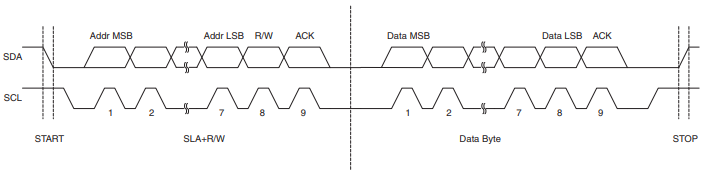
\includegraphics[width = 450pt]{Img/I2CTiming.png}
	\caption{I2C timing diagram}
	\label{fig:I2CTIming}
\end{figure}

Til udviklingen af masteren har et timing diagram over I2C protokollen, se \autoref{fig:I2CTIming}, været utrolig nyttig. Ved hjælp af dette diagram har gruppen kunne sende korrekte beskeder over I2C. 

For at have en så overskuelig kode som overhovedet muligt, er der blevet lavet funktioner der kan generere ACK, NACK, WAIT, START og STOP. Disse funktioner er så brugt i vores i2c\_master\_receive() funktion. Et Kodeudsnit af denne funktion kan findes nedenunder:

\newpage

\begin{lstlisting}
i2c_master_start();
while(transfer && i < 250)
{
	
	switch (i2c_master_status())
	{
		//SLA+R will be transmitted
		//ACK or NOT ACK will be received
		case 0x08:
		TWDR = address_r;
		i2c_master_ack();
		i2c_master_wait();
		break;
		
		// Data byte will be received and NOT ACK will be returned
		// Data byte will be received and ACK will be returned
		case 0x40:
		i2c_master_nack();
		i2c_master_wait();
		break;
		
		// Data byte will be received and NOT ACK will be returned
		// Data byte will be received and ACK will be returned
		case 0x50:
		data = TWDR;
		transfer = 0;
		break;
		
		// Repeated START will be transmitted
		// STOP condition will be transmitted and TWSTO Flag will be reset
		// STOP condition followed by a START condition will be transmitted and TWSTO Flag will be reset
		case 0x58:
		data = TWDR;
		transfer = 0;
		break;
	}
	i++;
}
i2c_master_stop();
\end{lstlisting}

Som det ses i koden bliver i2c\_master\_status() hele tiden tjekket på, for at finde ud af om slaven reagerer på nogle af kommandoerne fra masteren. Status funktion tjekker TWSR registeret og AND'er det med 0xF8, for at sætte de tre sidste bits til 0. I mega 2560 datablad kan der findes en tabel over hvad de forskellige status koder står for\cite{man:mega2560Kap24}. I kode udsnittet står de som kommentarer over hver case.

\subsection{I2C slave}
Ligesom masteren skal slave også initialiseres, ved at sætte nogle bestemte dataregistre op. TWAR registeret bestemmer slavens adresse, i vores tilfælde er den sat til 40. TWCR registeret bestemmer hvilken slave mode den skal sættes i, i vores tilfælde er det slave transmitter mode. Det vil sige at slaven kun skal kunne sende data til masteren, og ikke modtage data. 

Når slaven er sat op i transmitter mode, bliver der gjort brug af et interrupt, der trigger når i2c interfacet bliver brugt. Når et interrupt bliver triggered, køres vores interrupt rutine, som kan ses nedenunder:

\begin{lstlisting}
if(i2c_slave_addressed())
{

switch(i2c_slave_status())
{
// Own SLA+R has been received;
//ACK has been returned
case 0x60:
i2c_slave_ack();
break;

//Arbitration lost in SLA+R/W as
//Master; own SLA+R has been received;
//ACK has been returned
case 0x80:
data = TWDR;
i2c_slave_ack();
transfer = 0;
break;

// Data byte in TWDR has been
//transmitted; ACK has been received
case 0xA8:
TWDR = dataToSend; //data send to master
i2c_slave_ack();
break;

// Last data byte in TWDR has been
//transmitted (TWEA = 0)
// ACK has been received
case 0xC0:
transfer = 0;
i2c_slave_ack();
break;
}
}\end{lstlisting}

Interrupt rutinen minder meget om masterens receive funktion. Den tjekker hele tiden på status registeret(TWSR), for at holde styr på hvor langt den er i I2C processen. dataToSend indeholder en char med information om hvilken farve color sensoren har opfanget. 

\subsection{Test}
Til test af I2C, har vi gjort brug af en logic analyzer, som bruges til at afkode beskeder der sende med forskellige protokoller. Det har været en stor hjælp til at finde fejl i vores software. Blandt andet fandt vi ud af at hvis UART og I2C blev brugt samtidig, skabte det en stor nok forsinkelse i I2C protokollen. Dette skyldes at der ikke blev sendt et ACK på det rigtige tidspunkt. 

\begin{figure}[H]
	\centering
	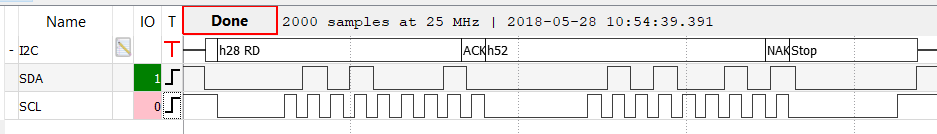
\includegraphics[width = 450pt]{Img/I2C_logic.png}
	\caption{Logic analyzer for I2C}
	\label{fig:I2C_Logic}
\end{figure}

På figuren ovenfor kan man se en perfekt I2C transmission. På figuren kan man se at et start condition, starter transmissionen, hvorefter adressen på slaven bliver sendt og at R/Wbit bliver sat højt, hvilket betyder READ. Derfter kommer dataen. I dette tilfælde bliver der sendt h52, hvilket i ASCII svarer til bogstavet 'R'. Et NACK kommer bagefter for at signallere at der ikke er mere data, hvorefter et stop condition blever genereret. Testopstillingen kan ses nedenunder.

\begin{figure}[H]
	\centering
	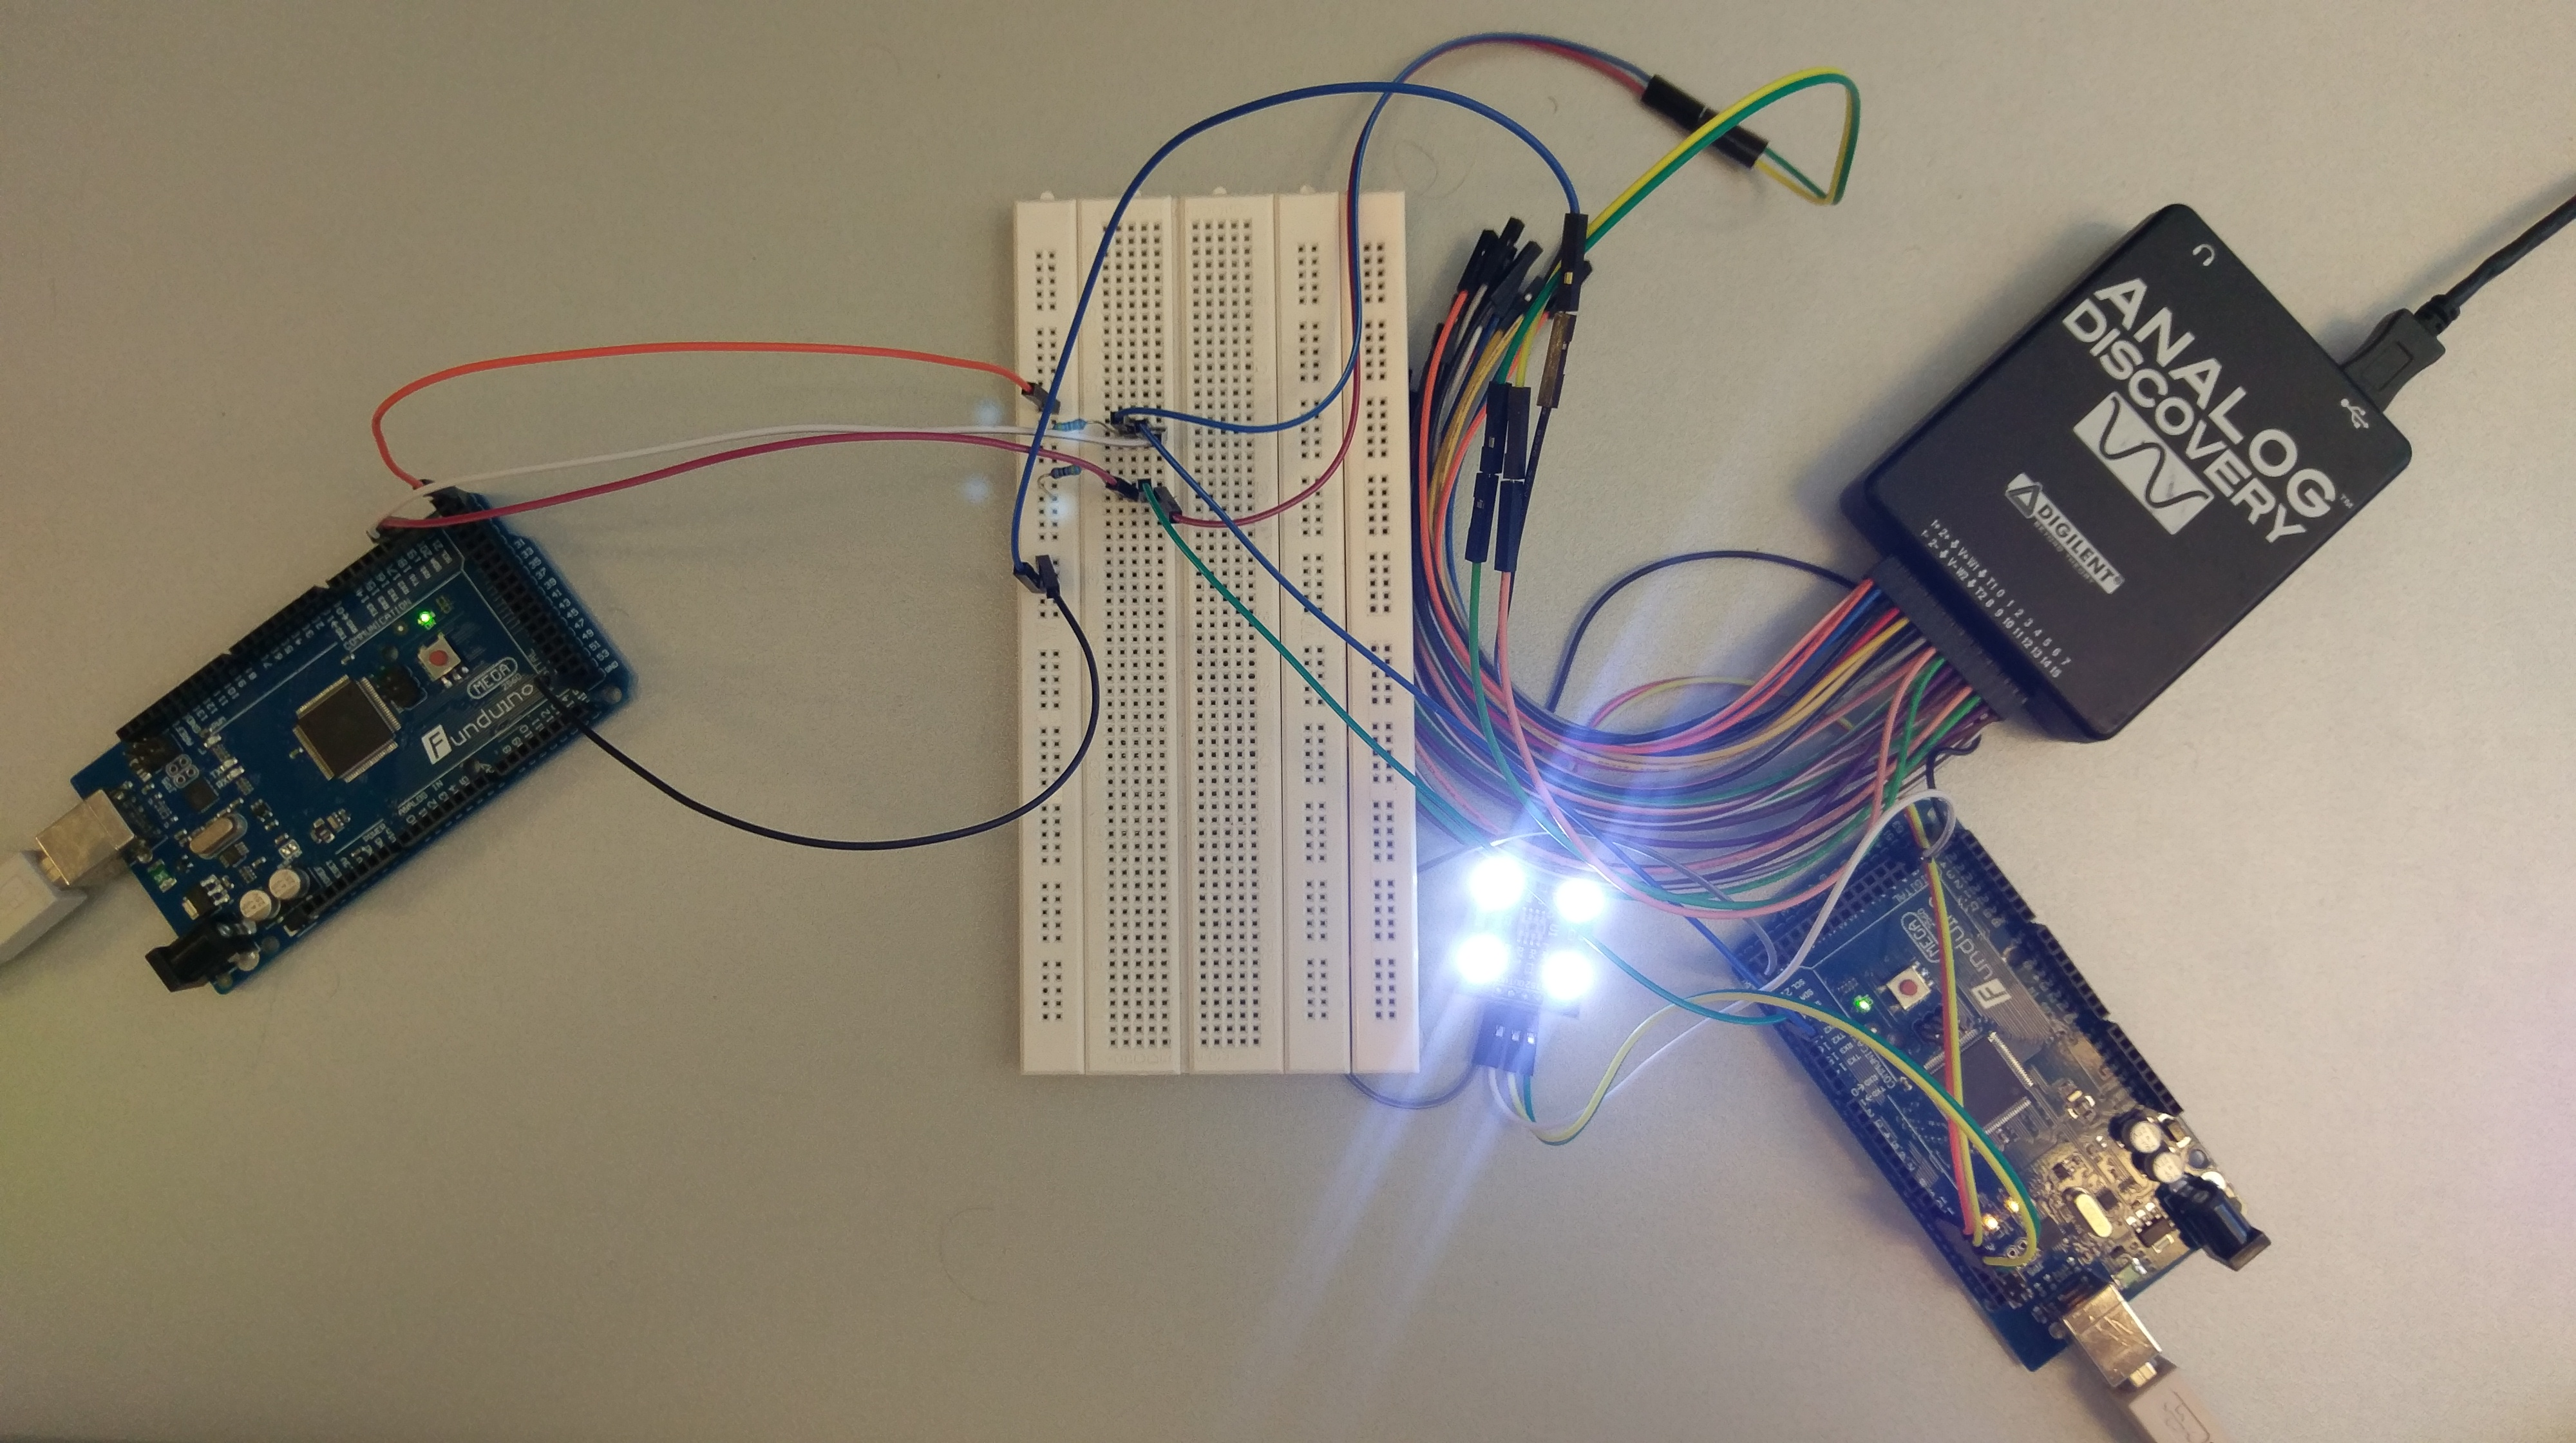
\includegraphics[width = 450pt]{Img/TestOpstilling.jpg}
	\caption{Test opstilling af I2C}
	\label{fig:I2C_Test}
\end{figure}


